%%%%%%%%%%%%%%%%%%%%%%%%%%%%%%%%%%
% Explanation of control regions
%%%%%%%%%%%%%%%%%%%%%%%%%%%%%%%%%%

\subsection{\texorpdfstring{$T$}{T} region \label{sec:boost_T_region}}

The $W$ tagger defined above will be used to select events in the signal region and in the TTJets
control region (see section~\ref{sec:Sregion} and \ref{sec:Tregion}). In both of those regions, we
expect to have real hadronically decaying $\W$ bosons, mainly coming from the $t\bar{t}+$jets
background. 


% The dominant background in the signal region is $t\bar{t}+$jets production. 
% We define the TTjets control region (denoted by \textsl{g1Mbg1W1LlmT100\_mdPhig0p5}, or simply $T$)
% with the following criteria on top of the baseline selection:
% \begin{itemize}
%  \item at least one CSV medium b-tagged jet,
%  \item at least one tagged W,
%  \item exactly one loose lepton (e or $\mu$)
%  \item transverse mass between the \ETm and the lepton, $m_T < 100\GeV$
%  \item $\Delta\phi_{min} > 0.5$
% \end{itemize}
% The main difference between this region and the signal region is the required presence of exactly
% one lepton. Here we also require $m_T < 100\GeV$ to reduce possible signal contamination. As can be
% seen from figure~\ref{fig:DataMC_T_mT}, $t\bar{t}+$jets production has a kinematic edge at the mass
% of the $W$ boson. This edge is not present for signal events where there is an additional
% contribution to the \ETm from the invisible neutralinos. 
% Indeed, looking at the same figure, we can see that the example signal point (grey histogram)
% extends out to high $m_T$ values. 
% All other cuts applied on top of the baseline selection are the same as for the signal region.
% 
% \begin{figure}[htbp]
% \centering
%  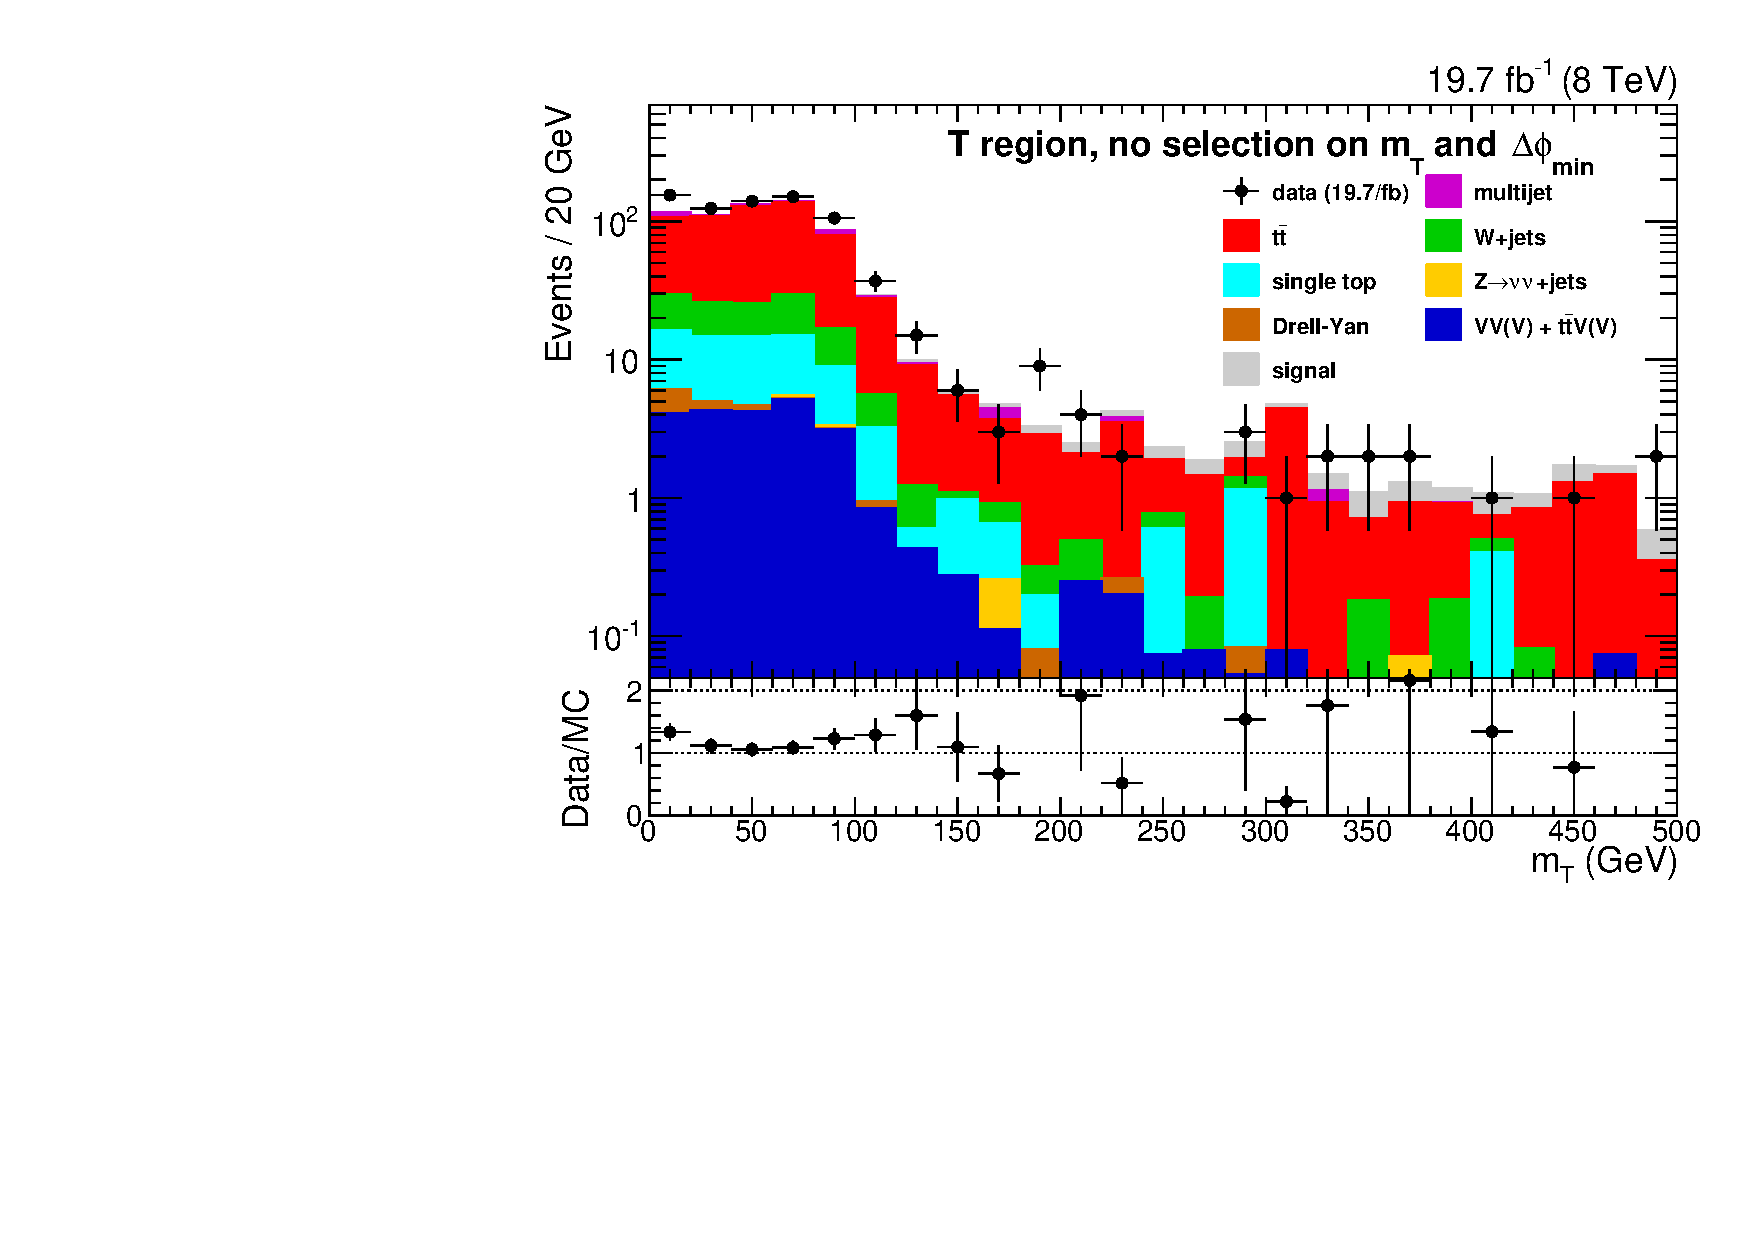
\includegraphics[width=0.49\textwidth]{figures/DataMC/DataMC_mT_g1Mbg1W1Ll_rebin}
%  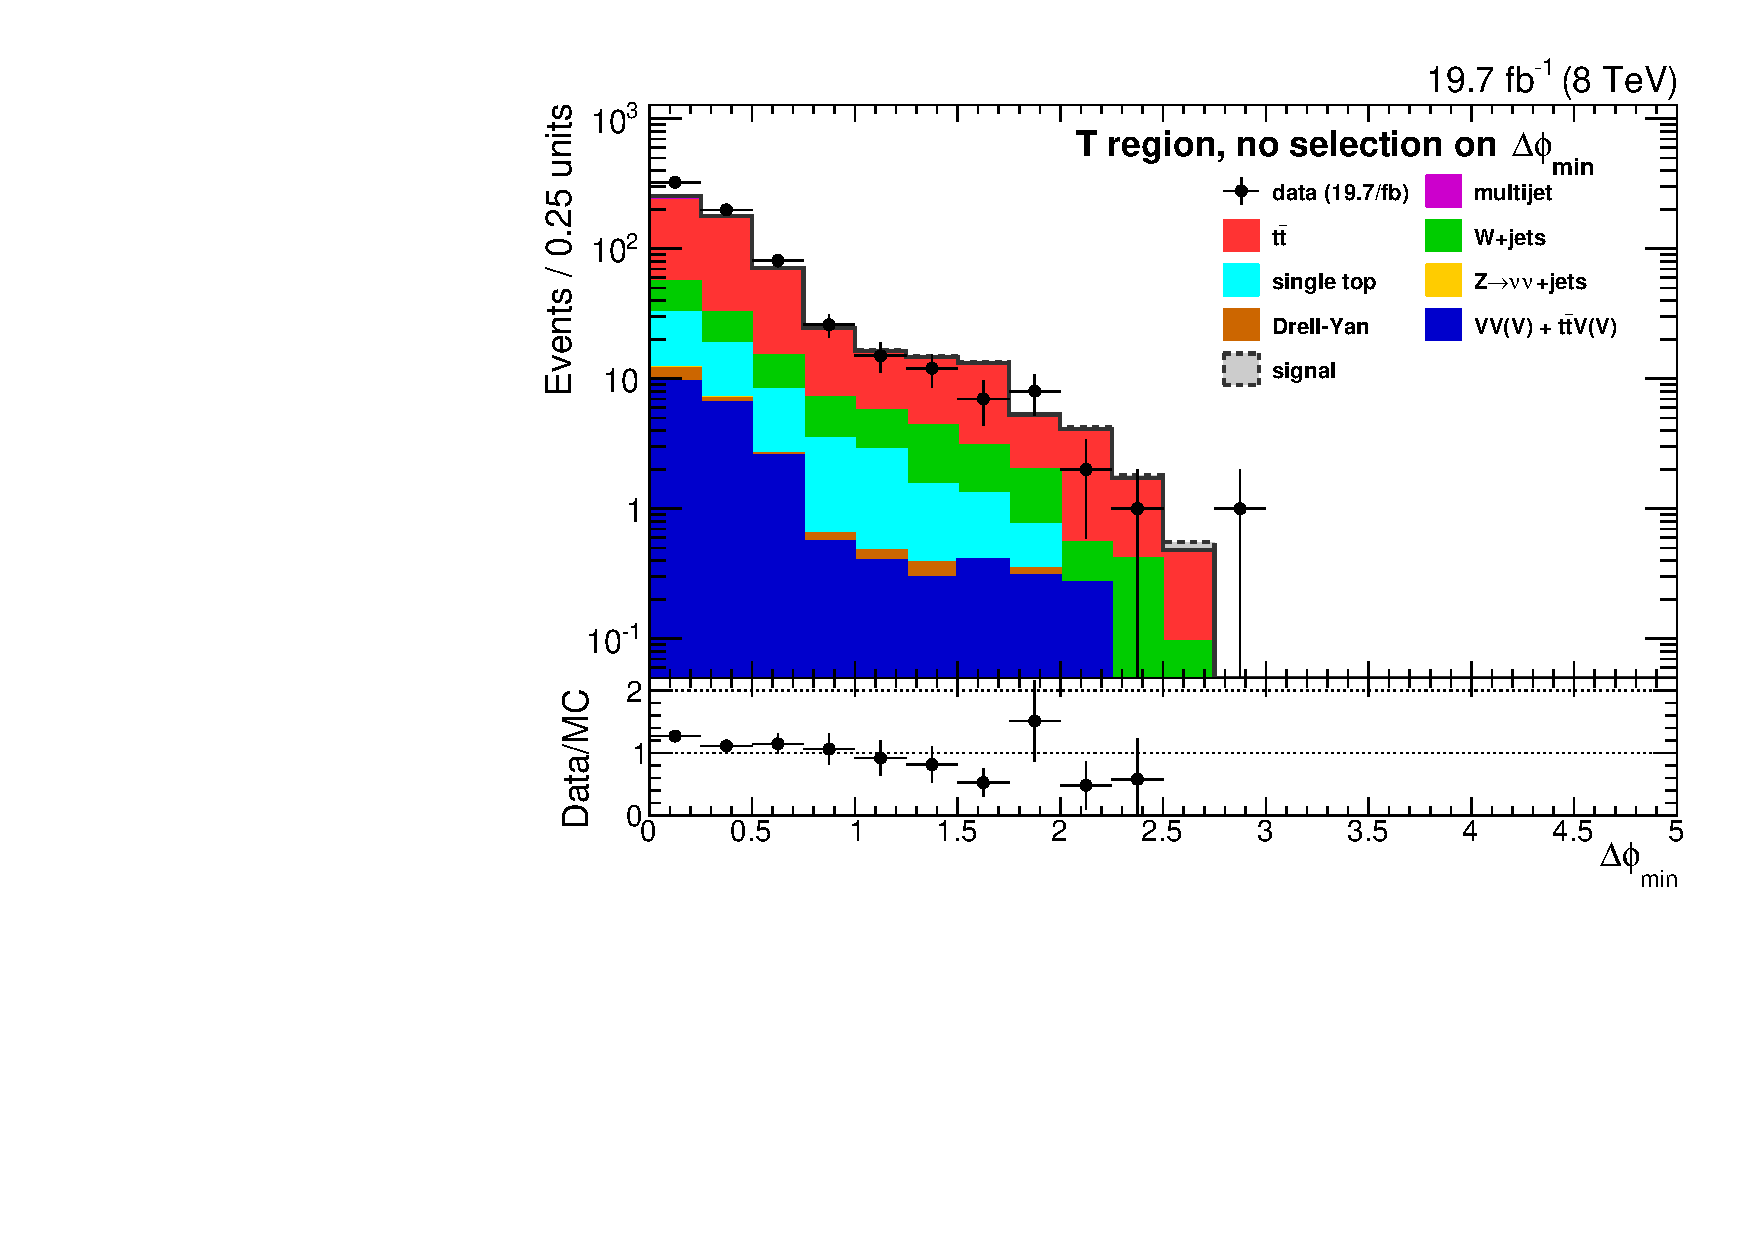
\includegraphics[width=0.49\textwidth]{figures/DataMC/DataMC_minDeltaPhi_g1Mbg1W1LlmT100_rebin}
% \caption{[left] Data/MC comparison plot of $m_T$ in the T region without the cut on $m_T$ and on
% $\Delta\phi_{min}$.
%    [right] Data/MC comparison plot of $\Delta\phi_{min}$ in the T region without the cut on
% $\Delta\phi_{min}$.
% \label{fig:DataMC_T_mT}}
% \end{figure}
% 
% The background composition as determined by simulation, is shown in tables~\ref{tab:cutflow} and
% \ref{tab:BG_comp_percent}. This region is about 80\% pure in $t\bar{t}+$jets and single top. 
% Comparisons between data and simulation for $M_R$ and $R^2$ in this region are shown in
% figure~\ref{fig:DataMC_TRegion_MR_R2_mdphig0p5}, and for various other basic quantities in
% figure~\ref{fig:DataMC_TRegion_mdphig0p5}. In figure~\ref{fig:Shape_TTJ_TvsS}, we show a comparison
% between the $M_R$ and $R^2$ shapes for TTjets simulation in the signal region versus the TTjets
% control region. The observed shapes are very similar. 
% 
% \begin{figure}[htbp]
% 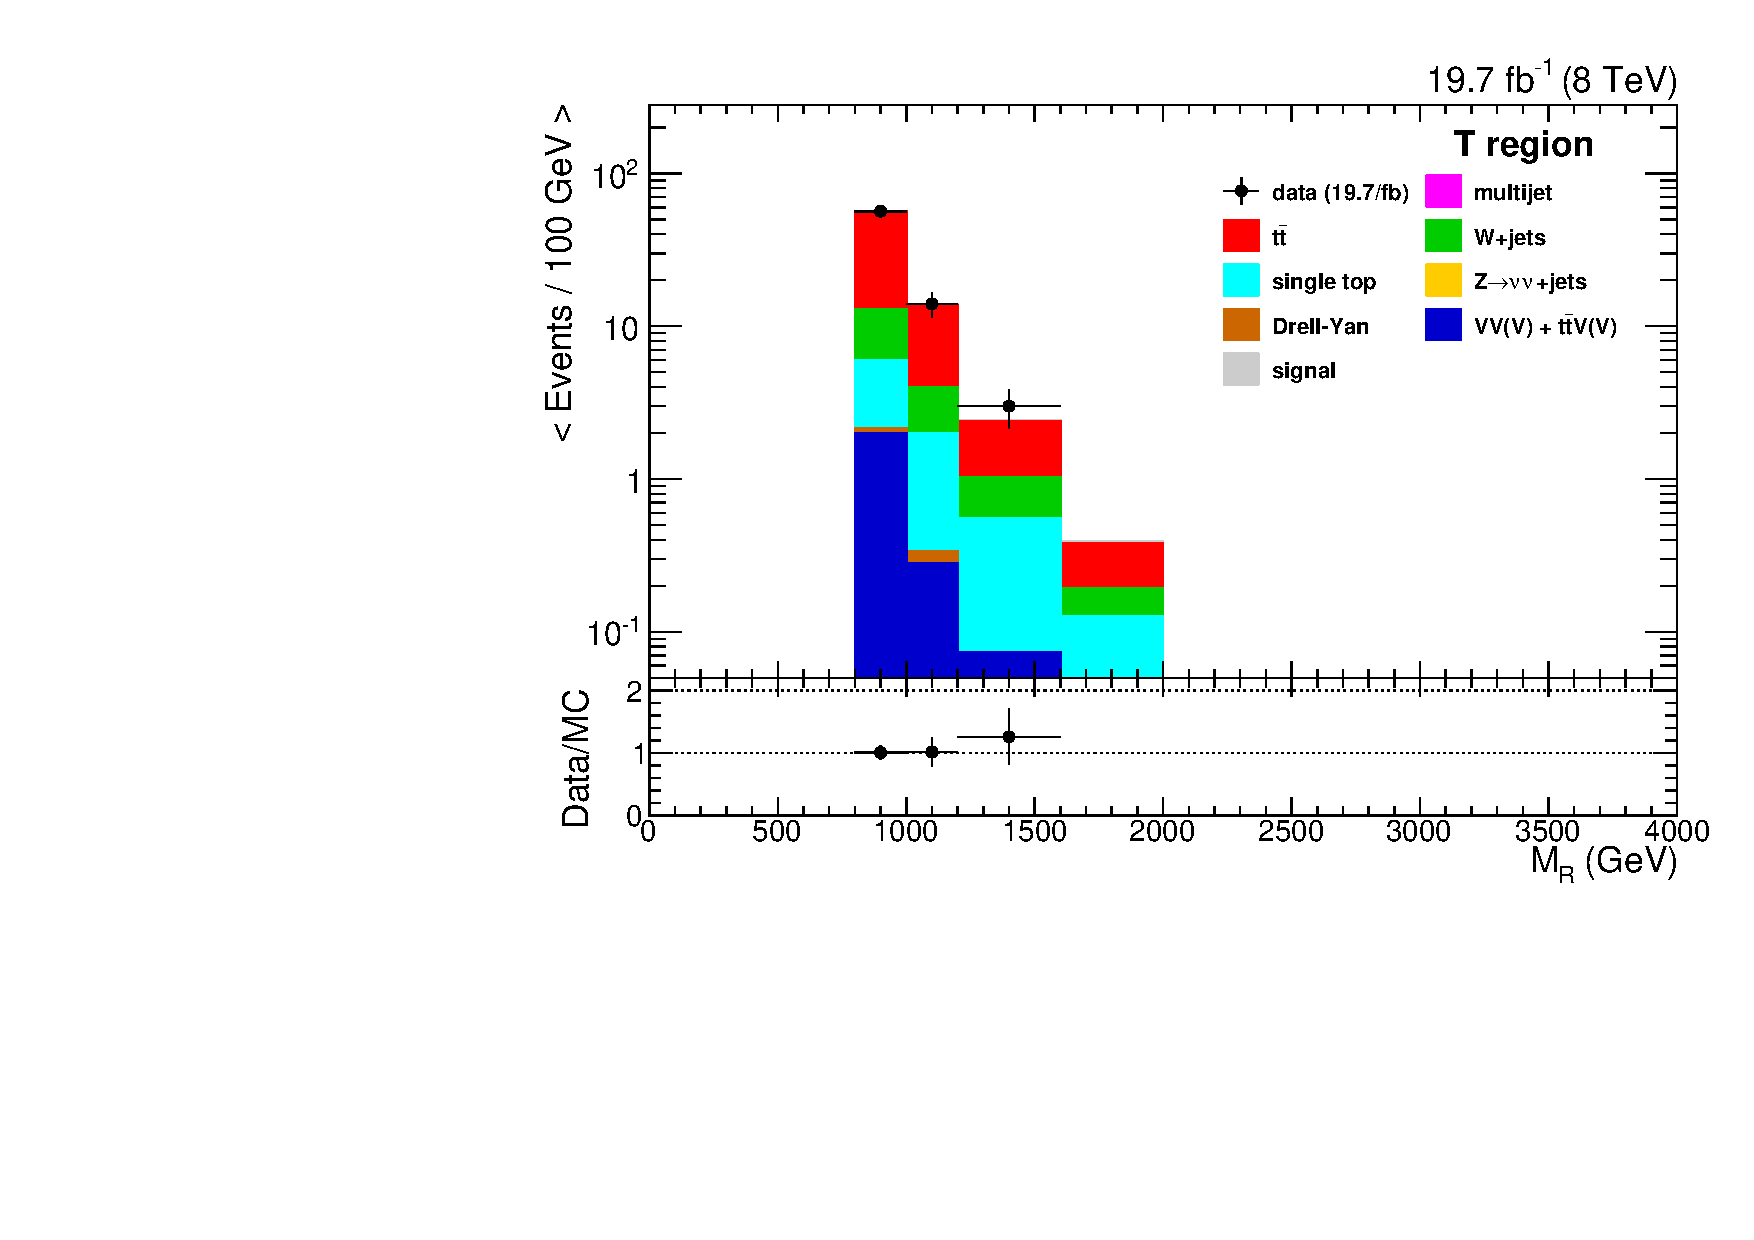
\includegraphics[width=0.49\textwidth]{figures/DataMC/DataMC_MR_g1Mbg1W1LlmT100_mdPhig0p5_width}
% 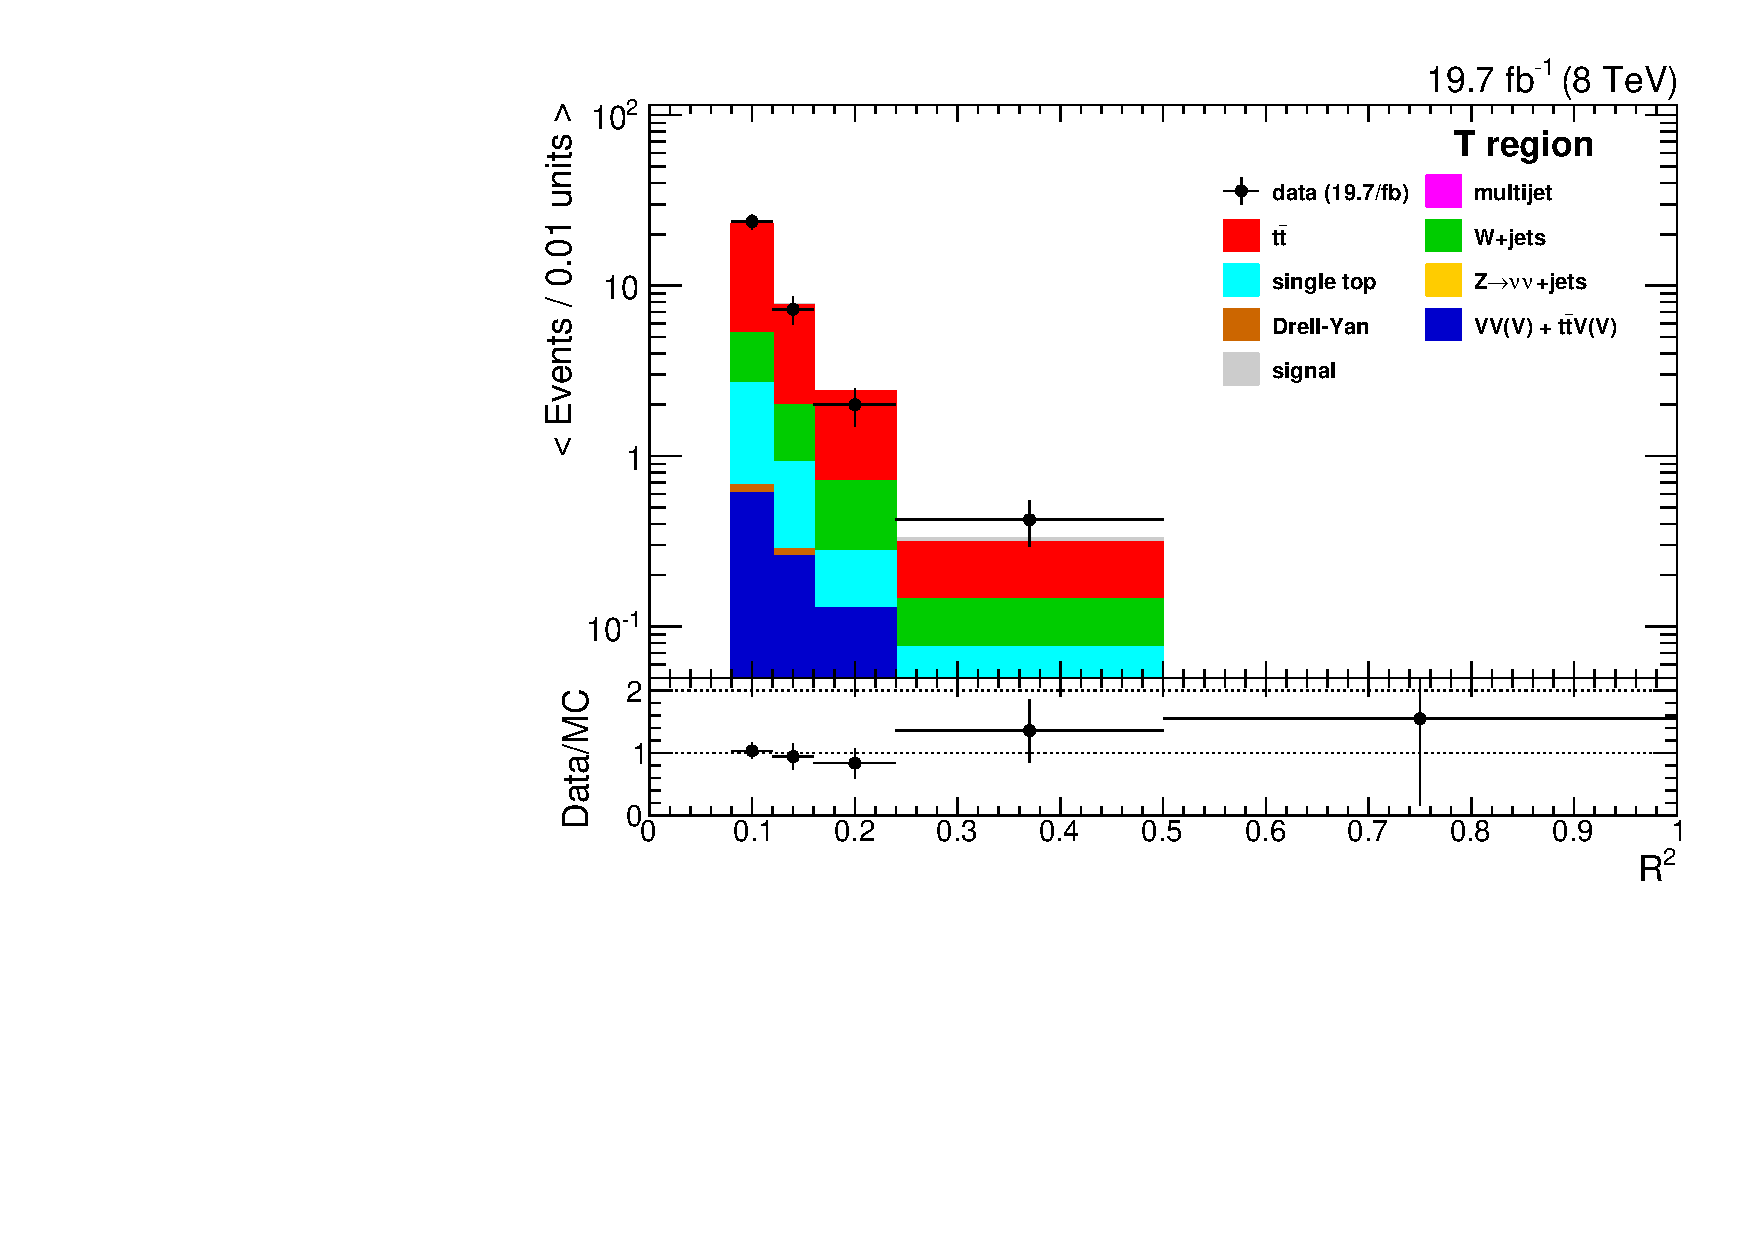
\includegraphics[width=0.49\textwidth]{figures/DataMC/DataMC_R2_g1Mbg1W1LlmT100_mdPhig0p5_width}
% \caption{Data/MC comparison plot of $M_R$ (left) and $R^2$ (right) in the TTjets control region.
% \label{fig:DataMC_TRegion_MR_R2_mdphig0p5}}
% \end{figure}
% 
% 
% \begin{figure}[p]
% \centering
%  \includegraphics[width=0.49\textwidth]{figures/DataMC/DataMC_njets_g1Mbg1W1LlmT100_mdPhig0p5}
%  \includegraphics[width=0.49\textwidth]{figures/DataMC/DataMC_nbjets_g1Mbg1W1LlmT100_mdPhig0p5}
% 
%  \includegraphics[width=0.49\textwidth]{figures/DataMC/DataMC_met_g1Mbg1W1LlmT100_mdPhig0p5}
%  \includegraphics[width=0.49\textwidth]{figures/DataMC/DataMC_jet1pt_g1Mbg1W1LlmT100_mdPhig0p5}
% 
%  \includegraphics[width=0.49\textwidth]{figures/DataMC/DataMC_jet2pt_g1Mbg1W1LlmT100_mdPhig0p5}
%  \includegraphics[width=0.49\textwidth]{figures/DataMC/DataMC_jet3pt_g1Mbg1W1LlmT100_mdPhig0p5}
% \caption{Data/MC comparison plot of various event quantities in the T region: 
% [top] jet multiplicity (left) and b-tagged jet multiplicity (right);
% [middle] missing transverse energy (left) and \pt of the highest \pt jet (right);
% [bottom] \pt of the second (left) and third (right) highest \pt jet. 
% \label{fig:DataMC_TRegion_mdphig0p5}}
% \end{figure}
% 
% \begin{figure}[htbp]
% \includegraphics[width=0.49\textwidth]{figures/Shapes/MR_comparison_TTJ_TvsS_mdphi}
% \includegraphics[width=0.49\textwidth]{figures/Shapes/R2_comparison_TTJ_TvsS_mdphi}
% \caption{Shape of $M_R$ (left) and $R^2$ (right) for $t\bar{t}+$jets simulation in the T region vs
% the S region. 
% \label{fig:Shape_TTJ_TvsS}}
% \end{figure}


%%%%%%%%%%%%%%%%%%%%%%%%%%%%%%%%%%%%%%%%%%%%%%%%%%%%%%%%%%%%%%%%%%%%%%%%%%%%%%%%%%%%%%%%%%%%%%%%

\subsection{\texorpdfstring{$Q$}{Q} region}

Another background in the signal region, is QCD multijet production, for which we have defined a
dedicated control region (section~\ref{sec:Qregion}). Multijet events do not have real $\W$ bosons;
any CA8 jet that passes the W tagger, is thus by definition a misidentified or \textit{fake} $\W$. 
For the QCD control region we define ``anti-tagged $W$'s'' ($aW$), in which we invert the
n-subjettiness cut but leave the other cuts the same. 
As we do not expect QCD events to have the two-prong jet-substructure of actual boosted $W$'s, this
will enhance the statistical power of the control region. 

% One of the main backgrounds in the signal region is QCD multijet production. In order to estimate
% this background, a dedicated control region (denoted by \textsl{0Lbg1uW0Ll\_mdPhi0p3}, or simply
% $Q$) is defined as follows: 
% \begin{itemize}
%  \item pass the baseline selection
%  \item have at least one anti-tagged $W$,
%  \item have no CSV loose b-tagged jets,
%  \item have no loose leptons,
%  \item have no isolated tracks.
%  \item $\Delta\phi_{min} < 0.3$
% \end{itemize}
% The differences with the signal region are the veto on b-jets, the requirement of an ``anti''-tagged
% W, and the change in the $\Delta\phi_{min}$ cut. Instead of only inverting the cut as applied in the
% signal region, we make it tighter to increase the purity of the selection. 
% 
% As was already mentioned in section~\ref{sec:Sregion}, we studied the $\Delta\phi_{min}$ and
% $\Delta\hat{\phi}_{min}$ variables as a means to further purify the QCD control region, beyond what
% was achieved by just requiring zero bjets and an anti-tagged W. 
% Our first studies showed a slightly better performance for the $\Delta\hat{\phi}_{min}$ variable,
% although with evolving selections (such as reducing the jet $|\eta|$ requirement from 3 to 2.4) the
% difference between both has basically disappeared. We show a comparison between data and simulation
% for both variables before cutting on them in figure~\ref{fig:DataMC_QRegion_mdphi}. 
% 
% The purity achieved with the current selection as listed above, is 90\% according to the simulation.
% In reality this percentage will be even higher, as simulation is seen to underpredict the data in
% this control region. This is a known feature of the QCD multijet simulation, and its normalisation
% to LO cross sections. 
% The full breakdown of the backgrounds according to simulation can be found in
% tables~\ref{tab:cutflow} and \ref{tab:BG_comp_percent}.
% 
% \begin{figure}[htbp]
% 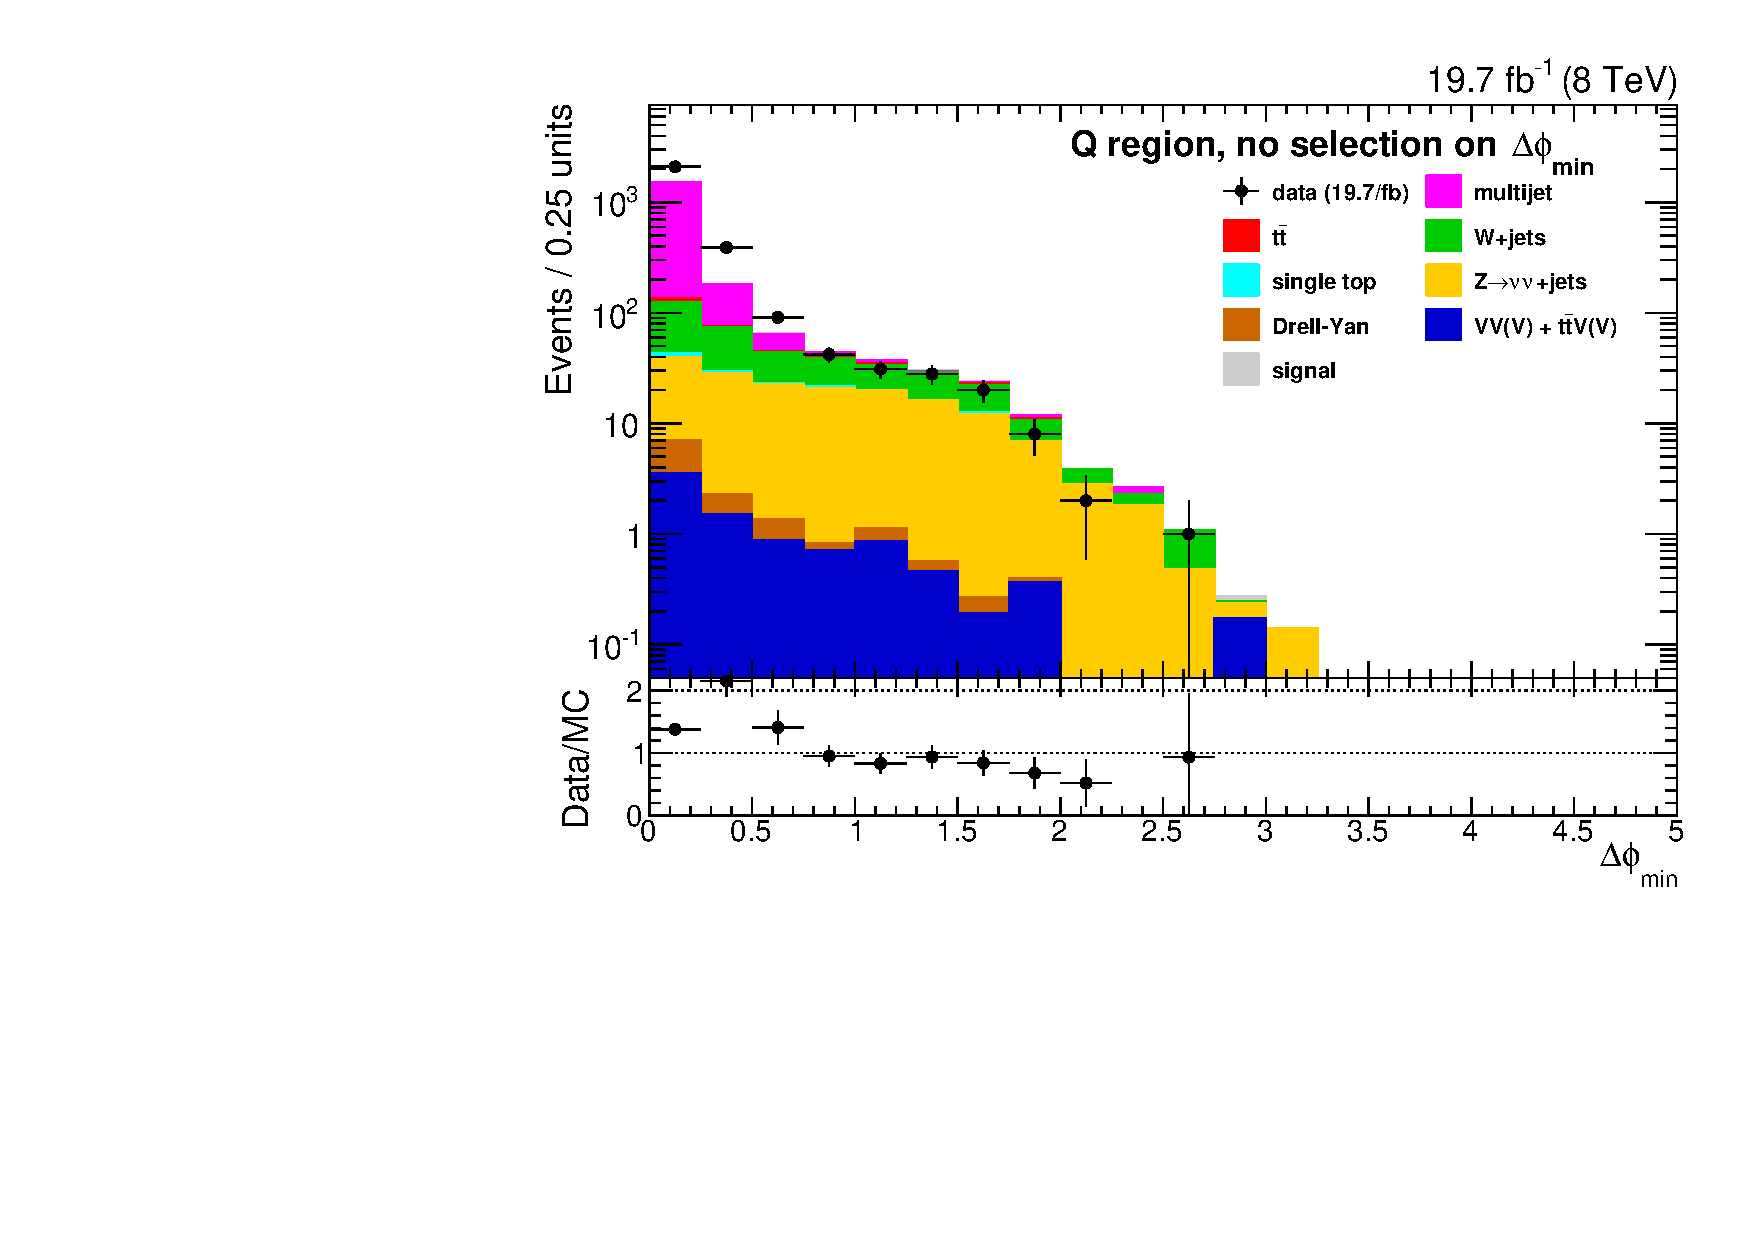
\includegraphics[width=0.49\textwidth]{figures/DataMC/DataMC_minDeltaPhi_0Lbg1uW0Ll_rebin}
% \includegraphics[width=0.49\textwidth]{figures/DataMC/DataMC_minDeltaPhiHat_0Lbg1uW0Ll}
% \caption{Data/MC comparison plot of $\Delta\phi_{min}$ (left) and $\Delta\hat{\phi}_{min}$ (right)
% in the QCD control region before cutting on either variable.
% \label{fig:DataMC_QRegion_mdphi}}
% \end{figure}
% 
% Comparisons between data and simulation in the $Q$ region for $M_R$ and $R^2$ are shown in
% figure~\ref{fig:DataMC_QRegion_MR_R2_mdphi0p3}, and for various other basic quantities in
% figure~\ref{fig:DataMC_QRegion_mdphi0p3}. In figure~\ref{fig:Shape_QCD_QvsS}, we show a comparison
% between the $M_R$ and $R^2$ shapes for QCD simulation in the signal region versus the QCD control
% region. As the statistical precision is quite limited for the QCD simulation in the signal region,
% we also show in figure~\ref{fig:Shape_QCD_QvsS_nomdphi} the comparison for the $Q$ and $S$ regions
% without selecting a particular $\Delta\phi_{min}$ region. The shape difference in this region is
% smaller than when the $\Delta\phi_{min}$ cut is applied. We will assign a 40\% systematic
% uncertainty on the QCD related quantities in the background prediction to account for the possible
% shape difference induced by the $\Delta\phi_{min}$ cut. 
% 
% \begin{figure}[htbp]
% 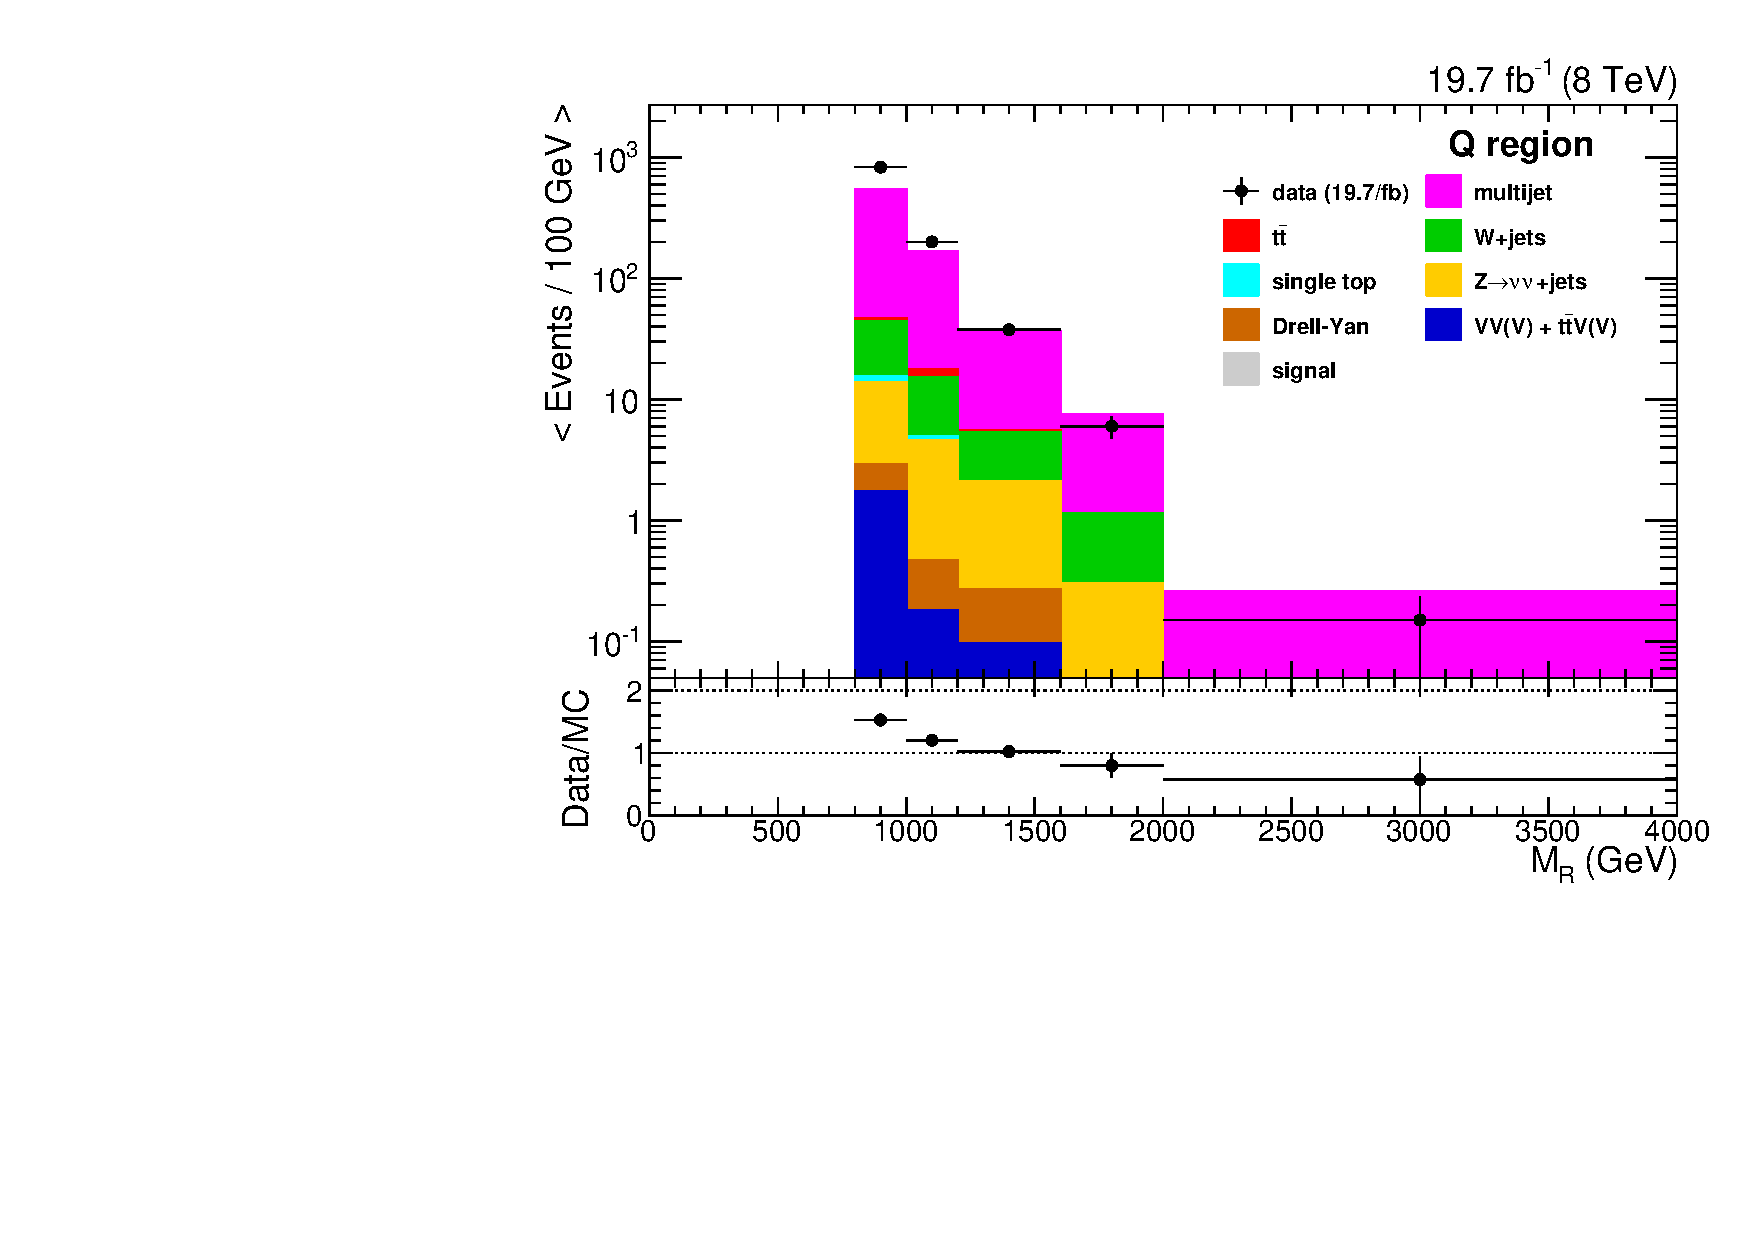
\includegraphics[width=0.49\textwidth]{figures/DataMC/DataMC_MR_0Lbg1uW0Ll_mdPhi0p3_width}
% 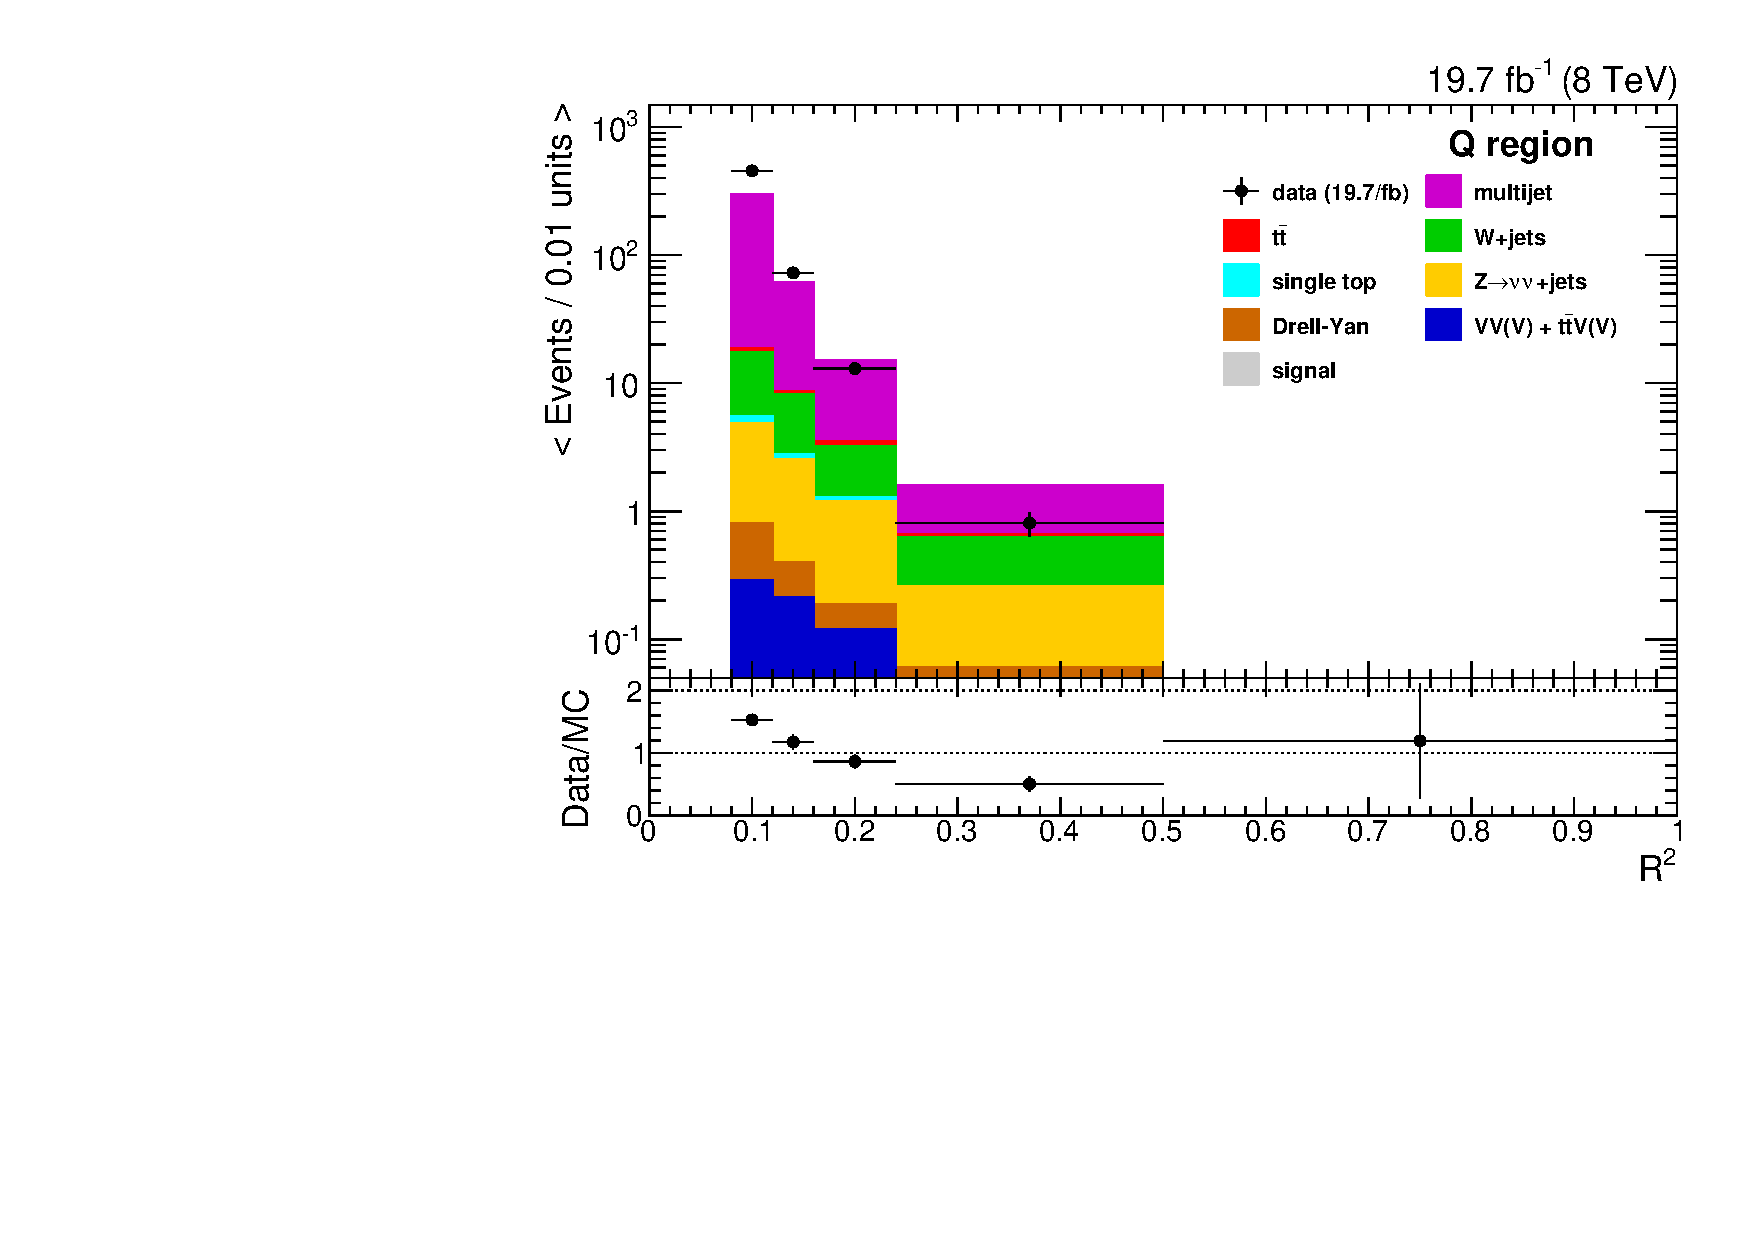
\includegraphics[width=0.49\textwidth]{figures/DataMC/DataMC_R2_0Lbg1uW0Ll_mdPhi0p3_width}
% \caption{Data/MC comparison plot of $M_R$ (left) and $R^2$ (right) in the QCD control region.
% \label{fig:DataMC_QRegion_MR_R2_mdphi0p3}}
% \end{figure}
% 
% 
% \begin{figure}[p]
% \centering
%  \includegraphics[width=0.49\textwidth]{figures/DataMC/DataMC_njets_0Lbg1uW0Ll_mdPhi0p3}
% 
%  \includegraphics[width=0.49\textwidth]{figures/DataMC/DataMC_met_0Lbg1uW0Ll_mdPhi0p3}
%  \includegraphics[width=0.49\textwidth]{figures/DataMC/DataMC_jet1pt_0Lbg1uW0Ll_mdPhi0p3}
% 
%  \includegraphics[width=0.49\textwidth]{figures/DataMC/DataMC_jet2pt_0Lbg1uW0Ll_mdPhi0p3}
%  \includegraphics[width=0.49\textwidth]{figures/DataMC/DataMC_jet3pt_0Lbg1uW0Ll_mdPhi0p3}
% \caption{Data/MC comparison plot of various event quantities in the Q region: 
% [top] jet multiplicity;
% [middle] missing transverse energy (left) and \pt of the highest \pt jet (right);
% [bottom] \pt of the second (left) and third (right) highest \pt jet. 
% \label{fig:DataMC_QRegion_mdphi0p3}}
% \end{figure}
% 
% \begin{figure}[htbp]
% \includegraphics[width=0.49\textwidth]{figures/Shapes/MR_comparison_QCD_QvsS_mdphi}
% \includegraphics[width=0.49\textwidth]{figures/Shapes/R2_comparison_QCD_QvsS_mdphi}
% \caption{Shape of $M_R$ (left) and $R^2$ (right) for QCD simulation in the Q region vs the S
% region. 
% \label{fig:Shape_QCD_QvsS}}
% \end{figure}
% \begin{figure}[htbp]
% \includegraphics[width=0.49\textwidth]{figures/Shapes/MR_comparison_QCD_QvsS_no_mdphi}
% \includegraphics[width=0.49\textwidth]{figures/Shapes/R2_comparison_QCD_QvsS_no_mdphi}
% \caption{Shape of $M_R$ (left) and $R^2$ (right) for QCD simulation in the Q region vs the S region
% with the requirement on  $\Delta\phi_{min}$ removed in both regions. 
% \label{fig:Shape_QCD_QvsS_nomdphi}}
% \end{figure}
% 

%%%%%%%%%%%%%%%%%%%%%%%%%%%%%%%%%%%%%%%%%%%%%%%%%%%%%%%%%%%%%%%%%%%%%%%%%%%%%%%%%%%%%%%%%%%%%%%%


\subsection{\texorpdfstring{$W$}{W} region}

Our final background in the signal region for which we have a dedicated control region, is
$\W(\rightarrow l\nu)$+jets. 
As the $\W$ boson decays leptonically, any events passing the signal selection must contain a CA8
jet that is misidentified as a boosted $\W$. 
We do not expect hadronically decaying $\W$ bosons to be a large background, as those events would
usually not come with $\cPqb$-jets, and would have very small missing energy. Even though we do not
explicitely require a minimal \ETm, our $R^2$ cut is highly correlated with \ETm, and induces
a minimal cut of around 100\GeV, as can be seen in figure~\ref{fig:DataMC_SignalRegion_mdphig0p5}.  
We have verified this assumption by checking the contribution of $\W(\rightarrow
q\bar{q}')+b\bar{b}$ using simulation, and found that no events pass our signal selection. 
For the $W$+jets control region, which is defined by requiring the presence of a lepton, we only
keep the mass window requirement to select CA8 jets that fake a boosted $\W$ boson. We will denote
these mass-tagged $\W$'s as $Y$. We do not use any cut on the n-subjettiness variables to increase
the number of events available in the control region. 

% 
% $W+$jets production is a relatively small contribution in the signal region, but we can still define
% a pure control region for it. 
% The $W+$jets control region (denoted by \textsl{0Lbg1Y1LlmT\_mdPhig0p5}, or simply $W$) is defined
% with the following criteria on top of the baseline selection:
% \begin{itemize}
%  \item no CSV loose b-tagged jets,
%  \item at least one ``Y'', \ie a CA8 jet with mass within the $W$ mass window, but without
% n-subjettiness cuts applied,
%  \item exactly one loose lepton (e or $\mu$)
%  \item transverse mass between the \ETm and the lepton, $30 < m_T < 100\GeV$
%  \item $\Delta\phi_{min} > 0.5$
% \end{itemize}
% The main difference between this region and the signal region is the required presence of exactly
% one lepton and the veto on b-jets. As for the T region, we require $m_T < 100\GeV$ to reduce
% possible signal contamination. We also require $m_T > 30\GeV$ to suppress contamination from
% multijet production. In figure~\ref{fig:DataMC_W_mT} we show the $m_T$ distribution in this region
% before applying the cut on $m_T$ or on $\Delta\phi_{min}$.
% 
% \begin{figure}[htbp]
% \centering
%  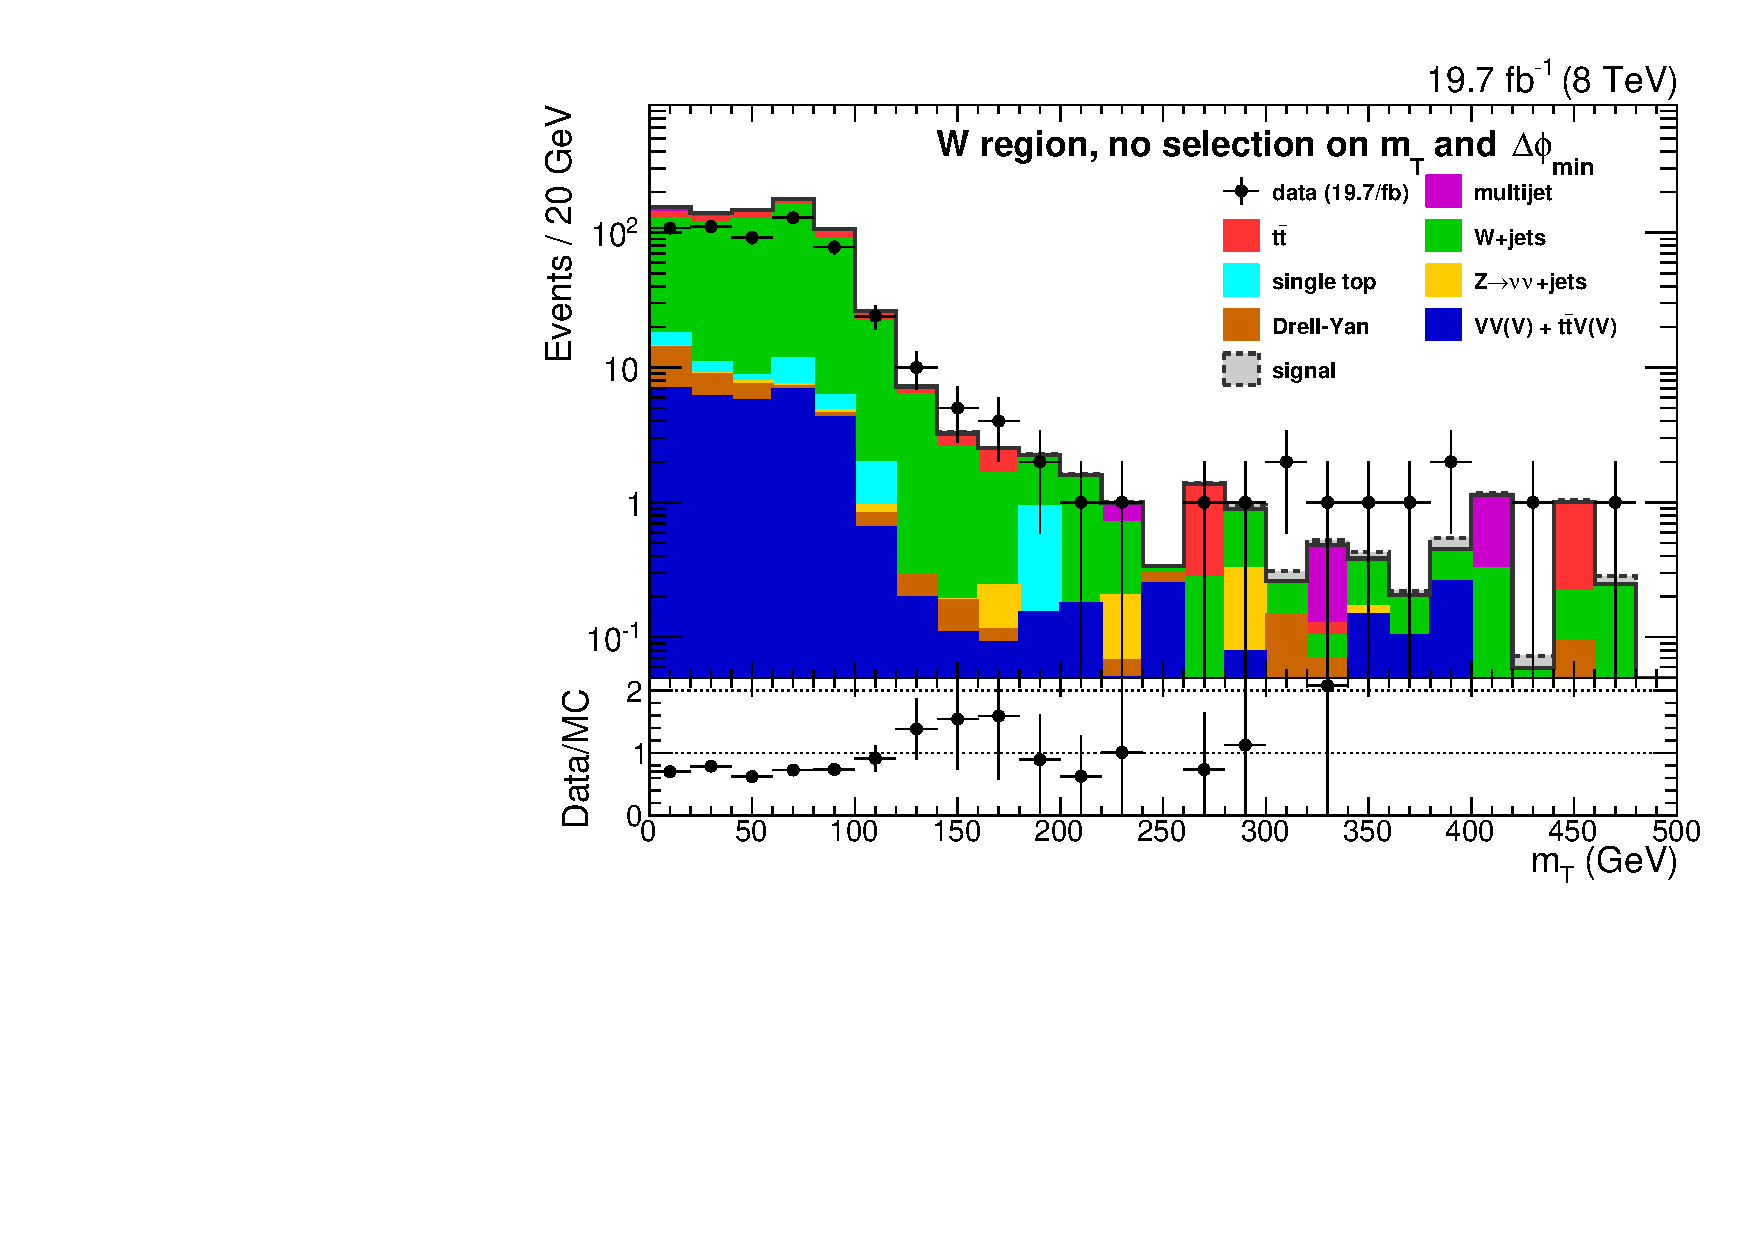
\includegraphics[width=0.49\textwidth]{figures/DataMC/DataMC_mT_0Lbg1Y1Ll_rebin}
%  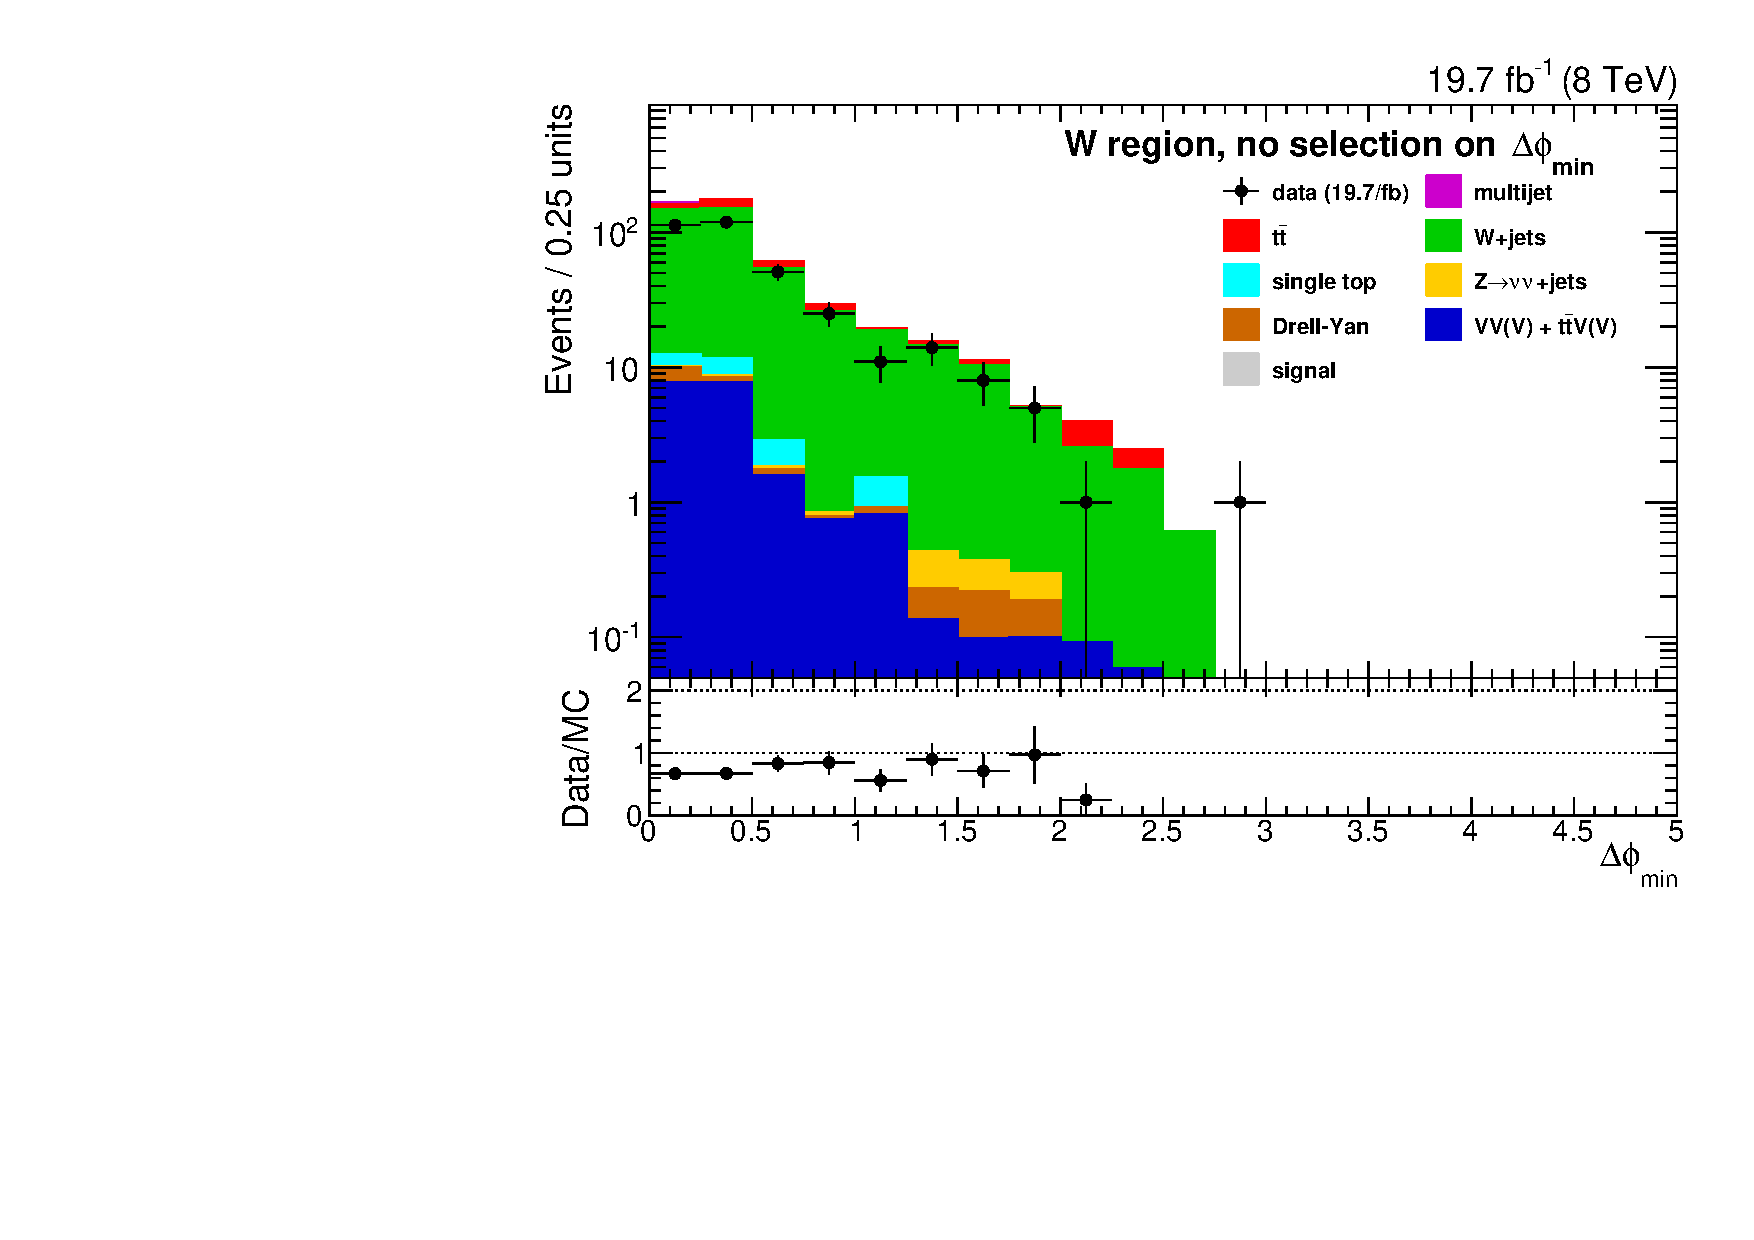
\includegraphics[width=0.49\textwidth]{figures/DataMC/DataMC_minDeltaPhi_0Lbg1Y1LlmT_rebin}
% \caption{[left] Data/MC comparison plot of $m_T$ in the W region without the cut on $m_T$ and on
% $\Delta\phi_{min}$.
%   [right] Data/MC comparison plot of $\Delta\phi_{min}$ in the W region without the cut on
% $\Delta\phi_{min}$.
% \label{fig:DataMC_W_mT}}
% \end{figure}
% 
% The background composition as determined by simulation is shown in tables~\ref{tab:cutflow} and
% \ref{tab:BG_comp_percent}. 
% Comparisons between data and simulation for $M_R$ and $R^2$ in this region are shown in
% figure~\ref{fig:DataMC_WRegion_MR_R2_mdphig0p5}, and for various other basic quantities in
% figure~\ref{fig:DataMC_WRegion_mdphig0p5}. In figure~\ref{fig:Shape_WJ_WvsS}, we show a comparison
% between the $M_R$ and $R^2$ shapes for Wjets simulation in the signal region versus the Wjets
% control region. The observed shapes are very similar. 
% 
% \begin{figure}[htbp]
% 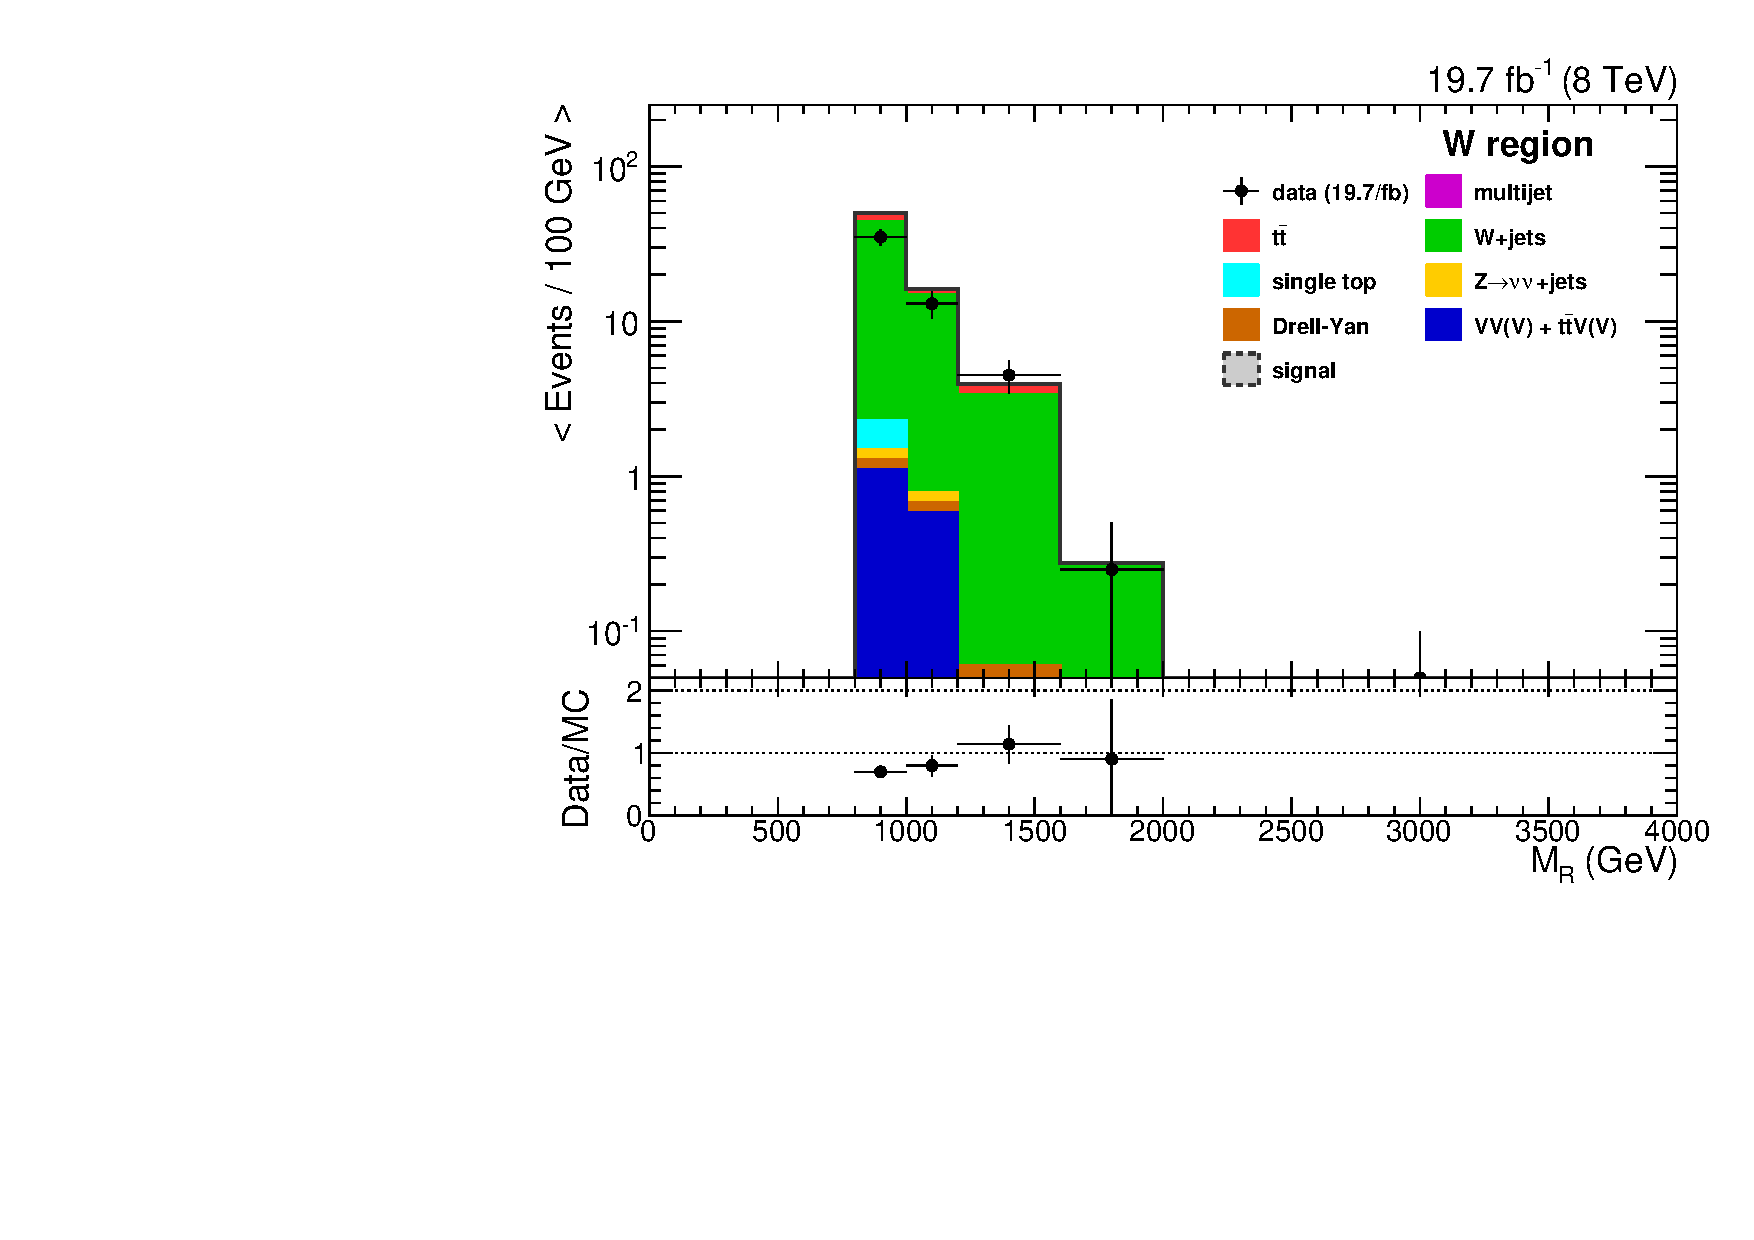
\includegraphics[width=0.49\textwidth]{figures/DataMC/DataMC_MR_0Lbg1Y1LlmT_mdPhig0p5_width}
% 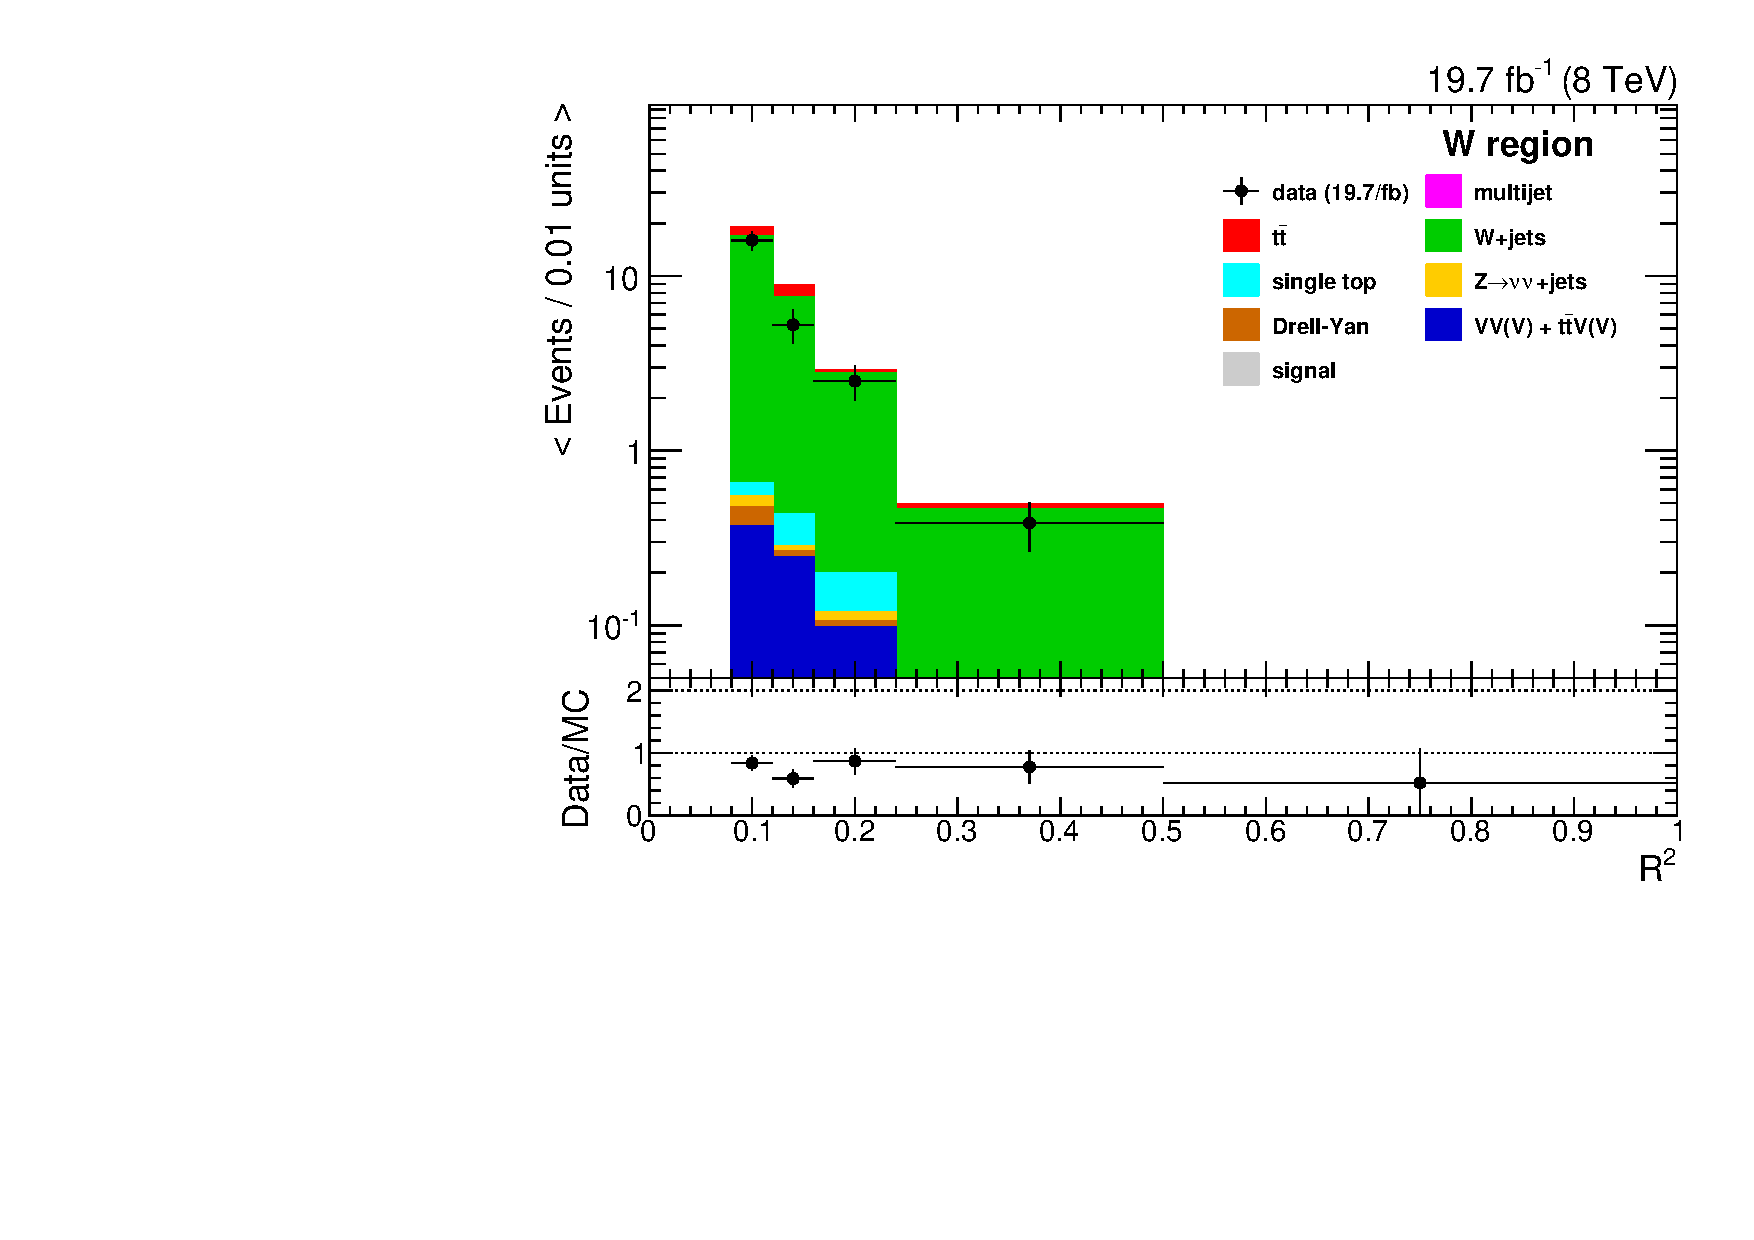
\includegraphics[width=0.49\textwidth]{figures/DataMC/DataMC_R2_0Lbg1Y1LlmT_mdPhig0p5_width}
% \caption{Data/MC comparison plot of $M_R$ (left) and $R^2$ (right) in the W region.
% \label{fig:DataMC_WRegion_MR_R2_mdphig0p5}}
% \end{figure}
% 
% 
% \begin{figure}[p]
% \centering
%  \includegraphics[width=0.49\textwidth]{figures/DataMC/DataMC_njets_0Lbg1Y1LlmT_mdPhig0p5}
% 
%  \includegraphics[width=0.49\textwidth]{figures/DataMC/DataMC_met_0Lbg1Y1LlmT_mdPhig0p5}
%  \includegraphics[width=0.49\textwidth]{figures/DataMC/DataMC_jet1pt_0Lbg1Y1LlmT_mdPhig0p5}
% 
%  \includegraphics[width=0.49\textwidth]{figures/DataMC/DataMC_jet2pt_0Lbg1Y1LlmT_mdPhig0p5}
%  \includegraphics[width=0.49\textwidth]{figures/DataMC/DataMC_jet3pt_0Lbg1Y1LlmT_mdPhig0p5}
% \caption{Data/MC comparison plot of various event quantities in the W region: 
% [top] jet multiplicity;
% [middle] missing transverse energy (left) and \pt of the highest \pt jet (right);
% [bottom] \pt of the second (left) and third (right) highest \pt jet. 
% \label{fig:DataMC_WRegion_mdphig0p5}}
% \end{figure}
% 
% \begin{figure}[htbp]
% \includegraphics[width=0.49\textwidth]{figures/Shapes/MR_comparison_WJ_WvsS_mdphi}
% \includegraphics[width=0.49\textwidth]{figures/Shapes/R2_comparison_WJ_WvsS_mdphi}
% \caption{Shape of $M_R$ (left) and $R^2$ (right) for $W+$jets simulation in the W region vs the S
% region. 
% \label{fig:Shape_WJ_WvsS}}
% \end{figure}

